\begin{center}
    \resizebox{0.45\textwidth}{!}{
        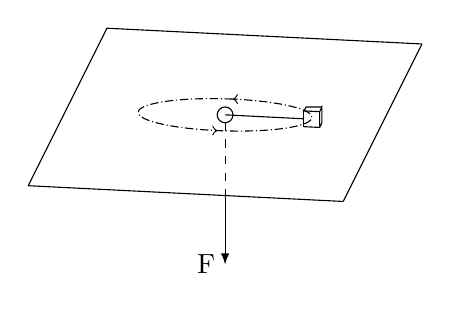
\begin{tikzpicture}
            \draw (0,0) to (4,-0.2);
            \draw (0,0) to (1,2);
            \draw (4,-0.2) to (5,1.8);
            \draw (1,2) to (5,1.8);
            \draw (2.5, 0.9) circle (0.1cm);
            \draw (2.5, 0.9) to (3.5, 0.85);
            \draw (3.5, 0.75) to (3.5, 0.95);
            \draw (3.7, 0.94) to (3.5, 0.95) to (3.53, 1) to (3.73, 1);
            \draw (3.5, 0.75) to (3.7, 0.74) to (3.7, 0.94) to (3.73, 1.00) to (3.73, 0.80) to (3.7, 0.74);
            \draw [black, densely dashdotted] plot [smooth cycle, tension=1] coordinates {(3.6, 0.85) (2.6, 1.1) (1.4, 0.95) (2.4, 0.7)};
            \draw[->] (2.4, 0.7) to ++(0.0004,-0.00002);
            \draw[->] (2.6, 1.1) to ++(-0.0004,+0.00002);
            \draw [black, dashed] (2.5, 0.8) to (2.5, -0.125);
            \draw [black, -latex] (2.5, -0.125) to (2.5, -1) node[left]{F};
        \end{tikzpicture}
    }
\end{center}
